\chapter{Probability} \label{sec:probability}
As stated in \cref{sec:introduction}, this section defines the concept of probability, which was proposed in \cite{kolmogorov}.
See \cref{fig:probability} and \cref{tab:probability}.

\begin{figure}[tb]
\centering
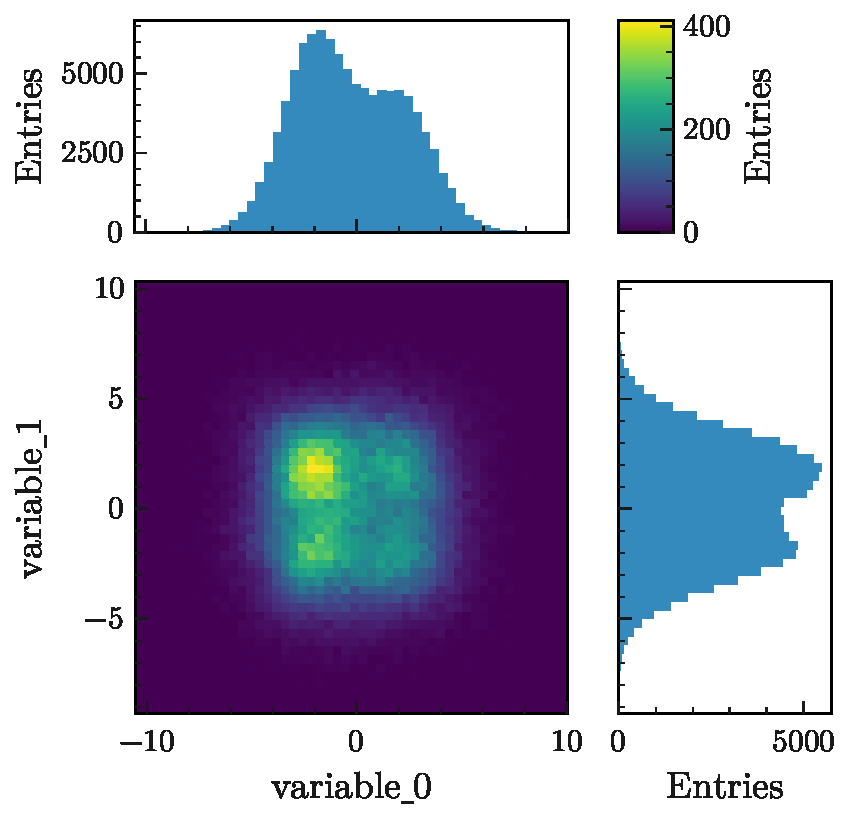
\includegraphics[width=0.75\textwidth]{figs/2d_hist_with_projections.pdf}
\caption{This is a caption.}
\label{fig:probability}
\end{figure}

\begin{table}[bt]
\caption{This is a caption.}
\begin{center}
\begin{tabular}{lll}
Name & Definition & Alternative names \\
\midrule
Purity & \textfrac{TP}{Predicted Positive}=\textfrac{TP}{TP+FP} & Precision \\
Efficiency & \textfrac{TP}{Real Positive}=\textfrac{TP}{TP+FN} & Recall, True Positive Rate \\
False Positive Rate & \textfrac{FP}{Real Negative}=\textfrac{TP}{FP+TN} & \\
\bottomrule

\end{tabular}
\end{center}
\label{tab:probability}
\end{table}
